\documentclass[conference]{IEEEtran}
\IEEEoverridecommandlockouts
% The preceding line is only needed to identify funding in the first footnote. If that is unneeded, please comment it out.
\usepackage{cite}
\usepackage{amsmath,amssymb,amsfonts}
\usepackage{algorithmic}
\usepackage{textcomp}
\usepackage{xcolor}
\usepackage{graphicx}
\usepackage{listings}

\graphicspath{ {./images/} }

\definecolor{codegreen}{rgb}{0,0.6,0}
\definecolor{codegray}{rgb}{0.5,0.5,0.5}
\definecolor{codepurple}{rgb}{0.58,0,0.82}
\definecolor{backcolour}{rgb}{0.95,0.95,0.92}

\lstdefinestyle{mystyle}{
    backgroundcolor=\color{backcolour},   
    commentstyle=\color{codegreen},
    keywordstyle=\color{magenta},
    numberstyle=\tiny\color{codegray},
    stringstyle=\color{codepurple},
    %basicstyle=\ttfamily\footnotesize,
    breakatwhitespace=false,         
    breaklines=true,                 
    captionpos=b,                    
    keepspaces=false,                 
    numbers=left,                    
    numbersep=3pt,                  
    %numberstyle=,                  
    showspaces=false,                
    showstringspaces=false,
    showtabs=false,                  
    tabsize=2
}

\lstset{style=mystyle}

\def\BibTeX{{\rm B\kern-.05em{\sc i\kern-.025em b}\kern-.08em
    T\kern-.1667em\lower.7ex\hbox{E}\kern-.125emX}}
\begin{document}

\title{Trabalho 1 - Filósofos Jantando\\Fundamentos de p. paralelo e distribuído}

\author{\IEEEauthorblockN{Guilherme Vieira, Lucca Demichei, Marcelo Rocha}
\IEEEauthorblockA{\textit{guilherme.camara@edu.pucrs.br, lucca.demichei@edu.pucrs.br, marcelo.rocha@edu.pucrs.br} \\
Escola Politécnica \\ PUCRS}}

\maketitle

\begin{abstract}
O trabalho trata da resolução do problema dos filósofos jantando, formulado por Dijkstra em 1965.
Três resoluções, na linguagem Java, são apresentados para a solução do problema.
\end{abstract}

\begin{IEEEkeywords}
filósofos, concorrência, Java, Dijkstra, thread, SMT.
\end{IEEEkeywords}

\section*{Introdução}

O problema dos filósofos jantando é um dos problemas clássicos usados para demonstrar os problemas existentes em um programa concorrente e foi elaborado por Dijkstra em 1965.\cite{wikipedia_2022}
O problema consiste em cinco filósofos jantando em uma mesa circular, sendo um prato para cada filósofo e um garfo entre cada prato, onde os filósofos pensam e comem simultaneamente.
\cite{baeldung_java}

\section{Funcionamento geral das soluções}

Testamos dois programas em Java \cite{baeldung_java} para resolver o problema dos filósofos.
As duas implementações são uma solução para o problema, rodam rapidamente, mas a versão com proteção de deadlock é mais rápida.
O motivo para isto é que a solução que faz tratamento do \textit{Deadlock} possui predefinido a ação de cada filosofo com uma melhor configuração,
enquanto na outra versão acontecem mais disputas pelo recurso, neste caso o garfo, ao longo da execução a tornando menos eficiente.

\section{Mecanismos usados na sincronização}
Nas soluções concorrentes, foram utilizadas threads para permitir que os cinco filósofos sejam transformados em processos que podem ser executados de forma simultânea.
Para sincronizar essas threads, foi usado um mecanismo denominado pelo autor como \textit{monitor}\cite{baeldung_java} que funciona como uma trava.
Esse sistema garante que enquanto um filósofo pega um garfo o outro filósofo ao seu lado não consegue acessar o mesmo garfo que está bloqueado.

\section{Como estes mecanismos são implementados na linguagem escolhida}

A classe \textit{Philosopher} implementa a interface \textit{Runnable} para permitir que executamos cada filósofo como uma thread separada.
No código em Java, para rodar um thread, precisamos sobreescrever o método \verb|run()| e depois declarar um thread e executar utilizando o método \verb|start()|.
Para sincronizar o acesso aos garfos é utilizado um bloco de código com a palavra reservada \textit{synchronized} que faz com que este bloco seja travado e o recurso, no caso o garfo, não possa ser acessado por outra thread (outro filósofo) enquanto estiver dentro do bloco.

\section{Como a solução evita Deadlock}

Para resolver o problema do Deadlock, o autor faz com que quatro filósofos peguem o garfo da sua esquerda, exceto o quinto filósofo que pegará o primeiro garfo a sua direita.
Fazer um dos cinco filósofos pegar na direção oposta dos demais, quebra o \textit{circular wait} que é um dos requisitos para acontecer o deadlock\cite{baeldung_java}.
O trecho de código \ref{code1}, que está dentro do loop que instancia os filósofos, apresenta a implementação dessa técnica para evitar o problema.

\lstinputlisting[label=code1, frame=single, firstnumber=57, language=Java, firstline=57, lastline=62, caption=Trecho de código que previne deadlock]{./codigos/PhilosopherDeadlock.java}

%\begin{verbatim}
%\begin{lstlisting}[language=Java, caption=código que previne Deadlock, label=code1]
%if (i == philosophers.length - 1)
%{
%  // The last philosopher picks up
%  // the right fork first
%  philosophers[i] = new Philosopher(rightFork, leftFork); 
%} else {
%  philosophers[i] = new Philosopher(leftFork, rightFork);
%}
%\end{lstlisting}
%\end{verbatim}

\section{Análise de tempo e solução sem concorrência}

Para que seja possível fazer uma comparação de tempo de execução fizemos uma versão sequencial, isto é, sem concorrência adaptada do código já existente.
O tempo foi medido usando o comando time do Linux que retorna o \textit{elapsed time} de qualquer programa quando utilizado antes na linha de execução do terminal.
As três versões foram executadas em um processador Intel\textsuperscript{\textregistered} Core\textsuperscript{\texttrademark} i5 3320M @ 2.60GHz com dois núcleos físicos e quatro threads lógicas, 8 GBs de memória principal e rodando Linux Ubuntu 20.04.5 LTS.

O tempo no qual chegamos foi calculado usando a média de três execuções e os resultados estão na tabela \ref{tabelaTempos}.

\begin{table}[h!]
\begin{tabular}{||c|c|c|c||c||}

\hline
\textbf{Versão}                                                    & \textbf{Tempo 1} & \textbf{Tempo 2} & \textbf{Tempo 3} & \textbf{Média} \\ \hline
Sequencial                                                         & 6,170            & 6,230            & 6,267            & \textbf{6,222} \\ \hline
\begin{tabular}[c]{@{}c@{}}Concorrente\\ simples\end{tabular}      & 3,825            & 4,158            & 3,582            & \textbf{3,855} \\ \hline
\begin{tabular}[c]{@{}c@{}}Protecão contra\\ deadlock\end{tabular} & 2,305            & 2,867            & 2,453            & \textbf{2,541} \\ \hline

\end{tabular}
\caption{Tempos de execução}
\label{tabelaTempos}
\end{table}

\section{Screenshots}

Seguem \textit{screenshots} da execução dos programas junto com o seu tempo de execução informado real pelo comando \verb|time| do Linux. As Figuras \ref{fig:linear}, \ref{fig:concorrente}, e \ref{fig:deadlock} são referentes à execução da versão linear, concorrente simples e protegida, respectivamente.

\begin{figure}[h!]
\caption{Execução do código linear}
\centering
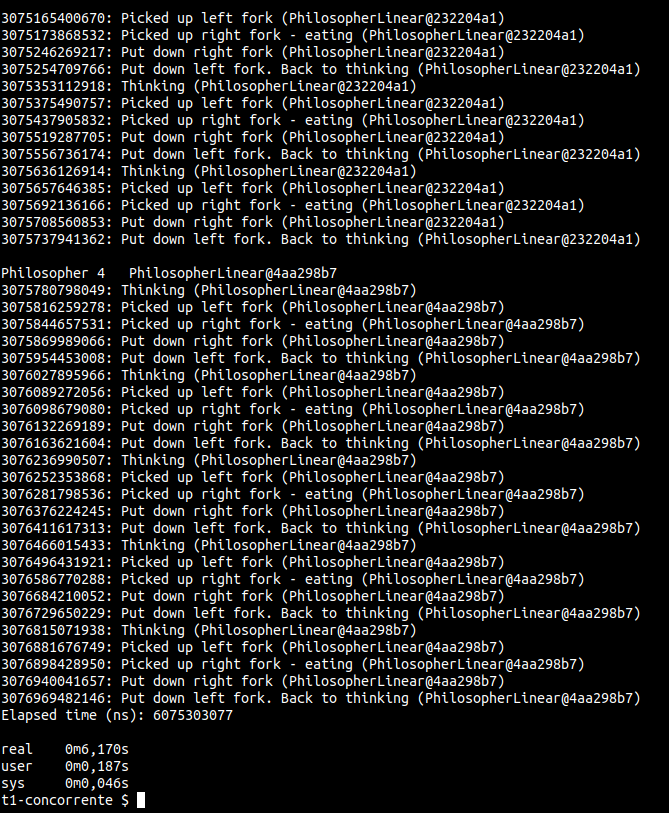
\includegraphics[width=8cm]{lin}
\label{fig:linear}
\end{figure}

\begin{figure}[h!]
\caption{Execução do código concorrente simples}
\centering
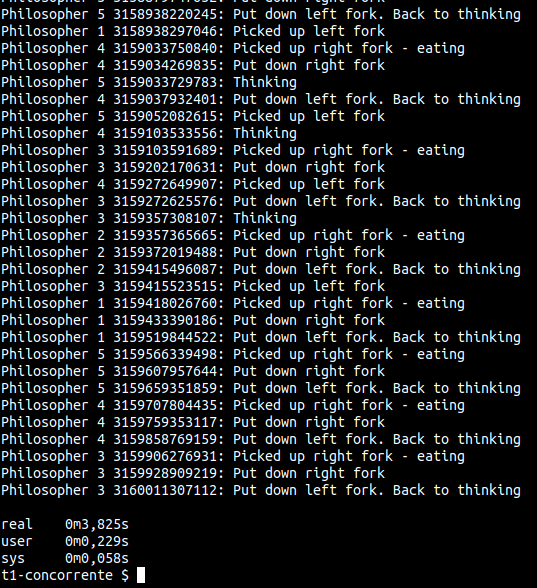
\includegraphics[width=8cm]{con}
\label{fig:concorrente}
\end{figure}

\begin{figure}[h!]
\caption{Execução do código com proteção contra deadlock}
\centering
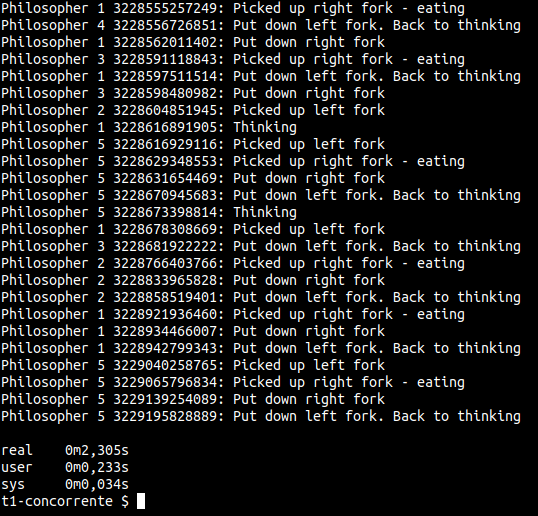
\includegraphics[width=8cm]{dea}
\label{fig:deadlock}
\end{figure}


\section{Código fonte}

% codigo linear
\lstinputlisting[language=Java, caption=Código Linear]{./codigos/PhilosopherLinear.java}

% codigo concorrente
\lstinputlisting[language=Java, caption=Código concorrente simples]{./codigos/PhilosopherConcurrent.java}

% codigo que evita deadlock
\lstinputlisting[language=Java, caption=Código que previne deadlock]{./codigos/PhilosopherDeadlock.java}

\bibliographystyle{IEEEtran}
\bibliography{ref} % Entries are in the ref.bib file

\end{document}